\chapter{Ambiente di Analisi}
Al fine di osservare il comportamento di SFA, e condurre l'analisi oggetto della Tesi, \`e stato costruito un ambiente atto a monitorare, in modo non intrusivo, il comportamento dell'algoritmo. \cite{monitoring}\\*
L'ambiente di analisi riproduce l'architettura software descritta nel capitolo 3, su una piattaforma \texttt{x86} equipaggiata con il sistema operativo \texttt{Windows 7}. 
\section{Principi di base}
L'ambiente di analisi deve essere tale da rispettare i principi della medesima. Non c'\`e interesse, nella fattispecie, a osservare il sistema a \emph{runtime}, ma lo scopo \`e unicamente quello di osservare il comportamento di SFA al variare dei dati in ingresso e dei parametri di configurazione.\\*
Vengono dunque escluse dalle campagne di analisi l'acquisizione delle misure dai sensori e la trasmissione degli output di SFA verso OBCU.\\*
L'intero processo di analisi viene condotto attraverso un software appositamente realizzato, il \emph{Rail Track Tool} (RTT).\\*
Il sistema di acquisizione e trasmissione delle misure viene opportunamente \emph{mockato} \cite{mocking} da una libreria usata da RTT, denominata \emph{SynthDataGen}, che fornisce allo stesso un \emph{framework} atto a simulare il comportamento dei sensori. RTT \`e dunque in grado di generare le misure che verosimilmente si otterrebbero sulla traccia in esame. 
\section{Software Impiegati}
\subsection{SensorFusionLib}
Libreria oggetto dell'analisi.
Essa \`e la stessa libreria che viene utilizzata da \emph{listener} nel sistema reale, ed \`e stata descritta nel capitolo 3.
\subsection{SynthDataGen}
Nell'ambiente di analisi, la libreria \emph{SynthDataGen} implementa la logica di \emph{interface-modules} nel sistema reale.\\*
\emph{SynthDataGen} utilizza le informazioni geografiche della traccia per generare i campionamenti di IMU e Odometro, tuttavia non supporta la generazione delle informazioni GPS.\\*
Nel sistema reale, le misure campionate da ciascun sensore sono caratterizzate da un \emph{rumore di misura} \cite{measnoise}, motivo per cui si palesa la necessit\`a di utilizzare SFA.\\*
Il rumore di misura \`e una caratteristica intrinseca di qualunque sensore, e viene modellato come una variabile aleatoria \emph{gaussiana} a media nulla il cui valore assunto viene sommato alle misurazioni. La variabile aleatoria che rappresenta il rumore di misura viene dunque completamente descritta dalla sua \emph{varianza} nel caso di generazioni univariate (Odometro), e dalla \emph{matrice di covarianza} nel caso di generazioni multivariate (IMU).\\*
L'ultima informazione che \`e necessario specificare per utilizzare \emph{SynthDataGen} \`e la frequenza di campionamento di ciascun sensore simulato, espressa in \emph{hertz}.
\begin{figure}[h]
	\centering
	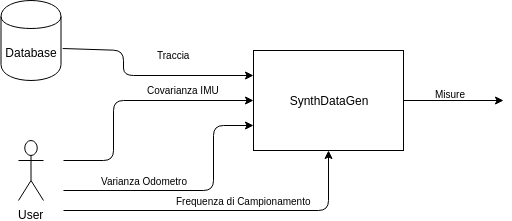
\includegraphics[width=0.7\linewidth]{img/SynthDataGen}
	\caption{Schema di SynthDataGen}
	\label{fig:SynthDG}
\end{figure}
\subsection{Rail Track Tool}
RTT \`e un software \emph{front-end} realizzato al fine di valutare le performance di SFA.\\*
Gli output di SFA non sono esclusivamente limitati alla stima della posizione del treno espressa come progressiva chilometrica; infatti date le caratteristiche dell'algoritmo, altre informazioni utili ai fini dell'analisi che esso fornisce sono:
\begin{itemize}
	\item Coordinate ECEF della posizione stimata del treno;
	\item Stima della velocit\`a proiettata lungo i 3 assi cartesiani;
	\item Errore commesso nella stima di posizione e velocit\`a.
\end{itemize}.
Il termine \emph{errore} indica la differenza, in valore assoluto, tra la stima prodotta e la misura reale.\\*
Nel sistema reale queste informazioni vengono semplicemente \emph{loggate} a scopi di debug o di \emph{monitoring online}, mentre nell'ambiente simulato da RTT queste informazioni vengono mostrate per intero. Non c'\`e dunque la necessit\`a di modificare il codice di \emph{SensorFusionLib} per valutare le misure di interesse, in quanto queste vengono calcolate per definizione dell'algoritmo. Quanto esposto dimostra la non intrusuvit\`a dell'attivit\`a di analisi.\\*
RTT include tra le sue dipendenze la libreria \emph{SensorFusionLib}, e ne sfrutta le relative \texttt{API} per alimentare SFA ed ottenere gli output dell'algoritmo; ed include \emph{SynthDataGen} per simulare il comportamento dei sensori.\\*
\begin{figure}[h]
	\centering
	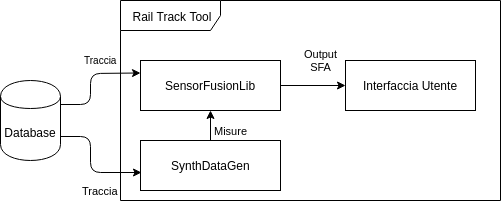
\includegraphics[width=0.7\linewidth]{img/RTTSchemaFull}
	\caption{Schema riassuntivo RTT}
	\label{fig:rttfull}
\end{figure}
\subsubsection{Interfaccia Utente}
All'avvio di RTT viene mostrata una finestra contenente l'interfaccia del software verso l'utente.\\*
\begin{figure}[h]
	\centering
	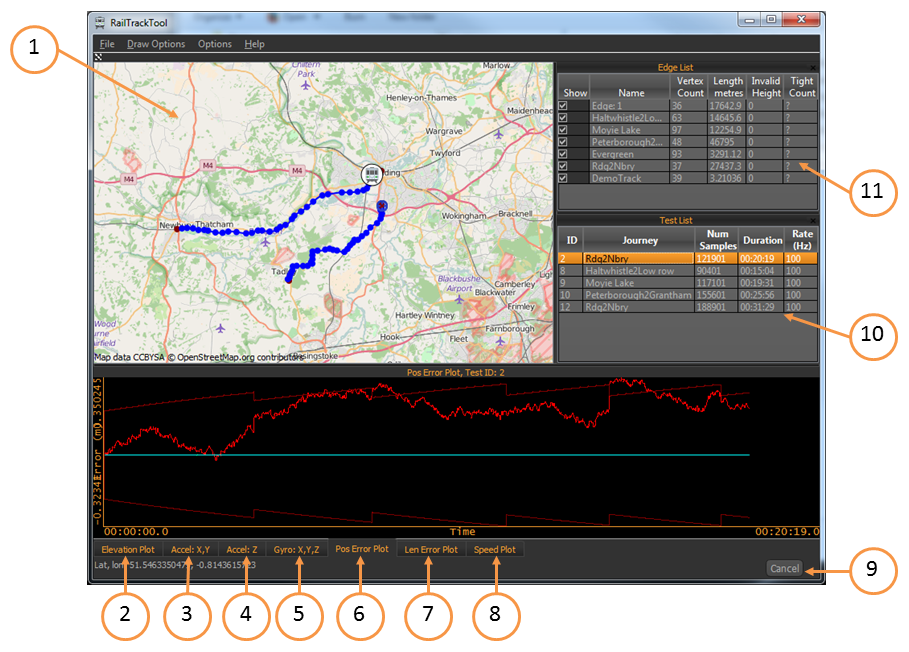
\includegraphics[height=7.8cm,width=\linewidth]{img/rtthci}
	\caption{Interfaccia RTT}
	\label{fig:rtt}
\end{figure}
\\*Gli elementi che compongono tale interfaccia sono:
\begin{enumerate}
\item \texttt{Slippy map}: Mappa che visualizza le traccie memorizzate, all'interno delle quali verr\`a mostrata la posizione del treno durante l'esecuzione di SFA;
\item \texttt{Elevation plot}: Grafico che mostra l'altitudine della traccia in funzione della progressiva chilometrica della stessa;
\item \texttt{Accel X,Y}: Grafico delle misure dell'accelerometro fornite a SFA, relative agli assi normale e tangenziale alla traccia selezionata;
\item \texttt{Accel Z}: Grafico delle misure dell'accelerometro fornite a SFA, relative all'asse verticale alla traccia selezionata; 
\item \texttt{Gyro X,Y,Z}: Grafico delle misure del giroscopio fornite a SFA, relative agli assi normale, tangenziale e verticale alla traccia selezionata;
\item \texttt{Pos error plot}: Grafico che riporta, in funzione del tempo, la stima dell'errore commesso nel predire la posizione del treno;
\item \texttt{Len error plot}: Come \texttt{Pos error plot}, ma l'errore \`e espresso rispetto alla progressiva chilometrica e non rispetto al vettore posizione;
\item \texttt{Speed Plot}: Grafico che mostra la stima della velocit\`a del treno come funzione del tempo;
\item \texttt{Cancel button}: Pulsante da premere se si ha la necessit\`a di interrompere una simulazione;
\item \texttt{Test List}: Storico delle analisi effettuate;
\item \texttt{Edge List}: Lista delle tracce memorizzate.
\end{enumerate}
\subsubsection{Monitoring con RTT}
Tramite un'apposita interfaccia interna a RTT, l'utente ha la possibilit\`a di definire i parametri generali con cui vengono generate le misurazioni, come ad esempio velocit\`a massima e frequenza di campionamento (figura \ref{fig:datagenerationconfig}).\\*
\begin{figure}[h]
	\centering
	\includegraphics[height=10cm,width=0.7\linewidth]{../Trainpositioning/train-positioning-tools/Documentation/UserGuide/DataGenerationConfig}
	\caption{Pannello di configurazione generale \emph{SynthDataGen}}
	\label{fig:datagenerationconfig}
\end{figure}\newpage
Un'altra interfaccia permette infine di definire le caratteristiche dei sensori simulati, come il rumore del processo di misura (figura \ref{fig:imuconfig}).\\*
\begin{figure}[h]
	\centering
	\includegraphics[height=4cm,width=0.7\linewidth]{../Trainpositioning/train-positioning-tools/Documentation/UserGuide/SensorModelConfig}
	\caption{Pannello di configurazione IMU simulato}
	\label{fig:imuconfig}
\end{figure}
\\*Definiti i parametri di configurazione \`e possibile selezionare una traccia, e simulare l'esecuzione di SFA.\\* Durante la simulazione, la posizione del treno stimata dall'algoritmo verr\`a visualizzata sulla mappa.\\*
\begin{figure}[h]
	\centering
	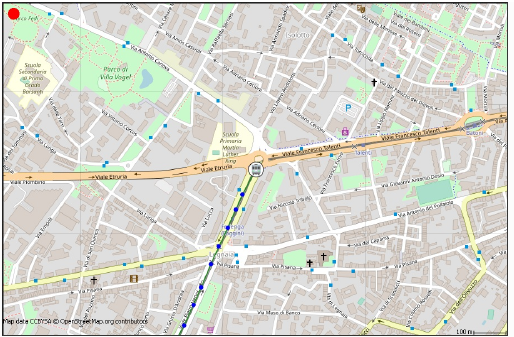
\includegraphics[width=0.7\linewidth]{img/trainmap}
	\caption{Posizione del treno mostrata sulla mappa}
	\label{fig:trainonmap}
\end{figure}
\\*Sui grafici nel pannello inferiore \`e possibile inoltre visualizzare i dati forniti in ingresso all'algoritmo, e gli errori commessi dallo stesso durante il processo di stima.\newpage
\begin{figure}[h]
	\centering
	\includegraphics[height=5cm,width=0.8\linewidth]{../Trainpositioning/train-positioning-tools/Documentation/UserGuide/DataPlotImuAccel.png}
	\caption{Grafico valori di accelerazione assi X e Y}
	\label{fig:imuxy}
\end{figure}
\begin{figure}[h]
	\centering
	\includegraphics[height=5cm,width=0.7\linewidth]{../Trainpositioning/train-positioning-tools/Documentation/UserGuide/DataPlotPosError.png}
	\caption{Grafico errore sulla stima della posizione}
	\label{fig:dataplotposerror}
\end{figure}
Al termine di ciascuna simulazione, RTT produce un report \texttt{HTML} contenente la sintesi dei principali risultati relativi alla simulazione appena effettuata.\\*
\subsubsection{Database Interface}
Come nel sistema reale, le informazioni geografiche relative alle tracce in esame sono memorizzate in un database. A differenza di quanto avviene nel sistema \emph{embedded}, in cui si utilizza un database \emph{sqlite}, nell'ambiente di analisi il database utilizzato \`e di tipo \emph{MySql}. Permane comunque inalterato lo schema logico del database (capitolo 3).\\*
Quanto esposto implica che all'atto di inizializzazione di SFA, RTT istanzi una connessione verso un database \emph{MySql}, implementata dalla classe concreta \texttt{MySqlDatabaseInterfaceEdges}.\\*